% -*- mode: noweb; noweb-default-code-mode: R-mode; -*-








\graphicspath{ {analysis/} }

\chapter{Analysis}
\label{cha:analysis}

% , eval=TRUE>>=

\begin{Schunk}
\begin{Sinput}
> options( prompt= " ", continue= " ", width= 60)
 options(error= function(){
   recover()
   options( prompt= "> ", continue= "+ ", width= 80)
 })
 source( "~/thesis/code/analysis.R")
 source( "~/thesis/code/peel.R")
 texWd <- "~/thesis/analysis"
 rasterWd <- "~/thesis/data/analysis"
 dataPath <- "~/thesis/data"
 setwd( rasterWd)
 overwriteRasters <- FALSE
                                         # studyArea used to work out RMSE
                                         # calcs and tables
 ##studyArea <- "thumb"
 studyArea <- "mlct"
                                         # bands are numbered from one but
                                         # classes from zero.  Used for stacks/brick
                                         # where bands correspond to classes
 peelBands <- peelClasses +1
                                         # mask and agland exported from GRASS
                                         # no need to mask or crop
 cusaMask <- raster( "mask_cusa.tif")
 cusaExtent <- extent( cusaMask)
 thumbExtent <- extent( -( 83 +30 /60), -( 82 +25 /60),
                           42 +55 /60,     44  +5 /60 )
                                         # default raster() output
                                         # has geographic proj, full extent
                                         # by default
 world <- raster()
 res(world) <- 5/60
 grid <- raster( cusaMask)
 grid[] <- cellsFromExtent( world, grid)
 grid <- mask( grid, cusaMask)
 if( studyArea == "thumb") {
   cusaMask <- crop( cusaMask, thumbExtent)
 }
 acresFile <- paste( "acres",
                    paste( studyArea, ".tif", sep=""),
                    sep="_")
 if( overwriteRasters) {
   acres <- area( cusaMask) *247.105381
   acres <- writeRaster( acres,
                        filename= acresFile,
                        overwrite= TRUE)
 } else acres <- raster( acresFile)
 agland <- stack( list.files( paste( dataPath, "agland", sep="/"),
                             patt= "(cropland|pasture).tif$",
                             full.names= TRUE))
 layerNames(agland) <- c("crop", "open")
 agland <- setMinMax( agland)
 if( studyArea == "thumb") {
   agland <- crop( agland, thumbExtent)
 }
 agg05 <-
   brick( list.files( dataPath,
                     patt= paste( studyArea, "_Amin_0.5_agg.tif", sep=""),
                     full.names= TRUE))
 layerNames( agg05) <- names( peelClasses)
 nomos05 <-
   brick( list.files( dataPath,
                     patt= paste( studyArea, "_Amin_0.5_nomosaic.tif", sep=""),
                     full.names= TRUE))
 layerNames( nomos05) <- c( names( peelClasses)[ -8], "total")
 agg1 <-
   brick( list.files( dataPath,
                     patt= paste( studyArea, "1_agg.tif", sep=""),
                     full.names= TRUE)) 
 layerNames( agg1) <- names( peelClasses)
 nomos1 <-
   brick( list.files( dataPath,
                     patt= paste( studyArea, "1_Amin_1_nomosaic.tif", sep=""),
                     full.names= TRUE))
 layerNames( nomos1) <- c( names( peelClasses)[ -8], "total")
 ## nlcd <- stack( paste( paste( dataPath, "nlcd", "nlcd", sep="/"), names( peelClasses[ -8]), "5min.tif", sep="_"))
 
 nlcd <- stack( sapply( names( peelClasses[ -8]),
                       function( cover) {
                         list.files( paste( dataPath, "nlcd", sep="/"),
                                    patt= paste( "nlcd", cover, "5min.tif$", sep="_"),
                                    full.names= TRUE)
                       }))
 nlcd <- setMinMax( nlcd)
 nlcd <- crop( nlcd, cusaMask,
              ##filename= paste( getwd(), "nlcd.tif", sep="/"),
              filename= "nlcd.tif",
              overwrite= TRUE)
 layerNames(nlcd) <- names( peelClasses[ -8])
 rasterNames <- c( "agland", "nlcd", "agg05", "agg1", "nomos05", "nomos1")
 dataSets <- sapply( rasterNames, function( n) eval( parse( text=n)))
 areas <- llply( dataSets,
 function( d) {
   res <- cellStats( d *acres, sum)
   names( res) <- layerNames( d)
   res
 })
 ## llply( areas, function( a) melt( a, value.name= deparse( substitute( a))))
 
 areasDf <- ldply( areas, function( a) melt( t( as.data.frame( a))))
 ## covers in columns
 ## areasCt <- cast( areasDf, .id ~ X2, subset= X2 != "total", sum, margins="grand_col")
 ## rownames( areasCt) <- areasCt[, ".id"]
 ## areasCt <- areasCt[, -1]
 ## areasCt[, c( names( peelClasses), "(all)")]
 
 ## covers in rows
 areasCt <- cast( areasDf, X2 ~ .id, subset= X2 != "total", sum, margins="grand_row")
 rownames( areasCt) <- areasCt[, "X2"]
 areasCt <- areasCt[, -1]
 areasCt <- areasCt[ c( names( peelClasses), "(all)"), rasterNames]
 
           
 
       
       
\end{Sinput}
\end{Schunk}


\begin{Schunk}
\begin{Sinput}
 local({
   colnames( areasCt) <- c( "Agland2000", "NLCD",
                           "\\pbox[c][][c]{3in}{Aggregated\\\\$A_{min}=0.5$}",
                           "\\pbox[c][][c]{3in}{Aggregated\\\\$A_{min}=1.0$}",
                           "\\pbox[c][][c]{3in}{No Mosaic\\\\$A_{min}=0.5$}",
                           "\\smallskip\\pbox[c][][c]{3in}{No Mosaic\\\\$A_{min}=1.0$}")
   print( xtable( areasCt / 10^6, 
                 caption= "Total Acreages by Map and Cover", 
                 label= "tab:areas",
                 digits= 1),
         add.to.row= list( 
           pos= list( 0, nrow( areasCt)),
           command= rep("\\noalign{\\smallskip}", times= 2)),
         size= "small",
         sanitize.colnames.function= function(x) x)
 })
\end{Sinput}
% latex table generated in R 2.12.2 by xtable 1.5-6 package
% Wed Mar 16 16:55:43 2011
\begin{table}[ht]
\begin{center}
{\small
\begin{tabular}{rrrrrrr}
  \hline
 & Agland2000 & NLCD & \pbox[c][][c]{3in}{Aggregated\\$A_{min}=0.5$} & \pbox[c][][c]{3in}{Aggregated\\$A_{min}=1.0$} & \pbox[c][][c]{3in}{No Mosaic\\$A_{min}=0.5$} & \smallskip\pbox[c][][c]{3in}{No Mosaic\\$A_{min}=1.0$} \\ 
  \noalign{\smallskip} \hline
water & 0.0 & 96.5 & 74.3 & 75.0 & 74.3 & 75.0 \\ 
  forest & 0.0 & 513.2 & 344.7 & 353.6 & 410.8 & 429.9 \\ 
  shrub & 0.0 & 420.1 & 358.7 & 341.8 & 387.2 & 368.0 \\ 
  open & 557.1 & 429.6 & 516.9 & 545.8 & 538.7 & 561.9 \\ 
  wetland & 0.0 & 95.0 & 26.0 & 11.0 & 26.0 & 11.0 \\ 
  crop & 446.5 & 310.8 & 378.9 & 369.6 & 495.4 & 488.1 \\ 
  urban & 0.0 & 102.8 & 27.3 & 29.8 & 27.3 & 29.8 \\ 
  mosaic & 0.0 & 0.0 & 232.9 & 237.0 & 0.0 & 0.0 \\ 
  barren & 0.0 & 24.5 & 32.8 & 28.9 & 32.8 & 28.9 \\ 
  (all) & 1003.7 & 1992.5 & 1992.5 & 1992.5 & 1992.5 & 1992.5 \\ 
   \noalign{\smallskip} \hline
\end{tabular}
}
\caption{Total Acreages by Map and Cover}
\label{tab:areas}
\end{center}
\end{table}\begin{Sinput}
 
 
 
\end{Sinput}
\end{Schunk}


After decomposing the mosaic class The MLCT indicates
495.4Ma (200.5Mha) of cropland for
$A_{min}=0.5$ and 488.1Ma (197.5Mha) for
$A_{min}=1.0$ in the cUSA in 2001. 

Pasture indicated by Aglands2000 appears to be a broader
classification than that of the NLCD's pasture class because much of
the grazing land east of the Mississippi river counted in the
Aglands2000 pasture map is absent in the NLCD pasture class.

Aglands2000 indicates roughly
Ma (Mha) of cropland.  The
inability of the MLCT data set to resolve rural transportation
networks, minor settlements, and small water or wetland features is a
major contribution to the surplus of cropland acreage indicated by the
MLCT.  Due to its greater resolution, ~30m vs. ~500m, the NLCD is
better suited at discerning developed areas in rural landscapes
ranging from rural roads to farmsteads to small communities that do
not show up in the MLCT data. There is a total area of roughly 74 Ma
(30 Mha) of development remaining after subtracting the MLCT urban
class from all developed classes in the NLCD where the NLCD shows
greater development after they have both been aggregated to the
5-arcmin grid. Applying this area as an offset to the cropland area in
Aglands2000 brings us closer to the expected acreage under cultivation
in 2001, although this assumes that all of that development intersects
with MLCT cropland area.


The purpose for processing the MLCT for two values of $A_{min}$ as
described in the previous chapter is to evaluate whether or not
information from the secondary cover type contributes positively to
the accuracy of the data set we seek to synthesize.  The primary
objective of this synthesis is to achieve accuracy in cropland
distribution.  Because the cropland layer in the Agland2000 data set
is derived from county-level production census statistics we adopt
this as the ground truth and will endeavor to adjust our product
accordingly.  Although MLCT overstates cropland acreage for both
$A_{min}=0.5$ and $A_min=1.0$ the discrimination among the two is made
by the distribution of errors rather than the aggregate error.

\missingfigure{error map for ``nomos'' vs. Agland2000 crop}

These maps show the cell-by-cell differences between the MLCT-derived
data set that we have calculated after mosaic decomposition and the
Agland2000 cropland map.  TO summarize and compare these errors we
calculate the root of the mean squared error (RMSE) given by:

$$
\operatorname{RMSE}=\sqrt{\frac{\sum_{i=1}^{n}(\hat\theta_i-\theta_i )^2}{n}}
$$

where $\hat\theta_i$ are the predictions derived from the respective
MLCT derivations and $\theta_i$ are the observations taken from the
Agland2000 data set.


\begin{Schunk}
\begin{Sinput}
 rmseDf <- ldply( list("nomos05", "nomos1"),
                 function( brickName) {
                   rmseRast( getPeelBand( get( brickName), "crop"),
                            unstack( agland)[[1]])
                 })
 rmseDf <- cbind( c( 0.5, 1.0), rmseDf)
 colnames( rmseDf) <- c( "$A_{min}$", "RMSE")
 
 
\end{Sinput}
\end{Schunk}



\begin{Schunk}
\begin{Sinput}
 print( xtable( rmseDf,
               caption= "RMSE, MLCT vs. Agland2000 crop",
               label= "tab:rmse",
               digits= c( 0, 1, 3)),
       include.rownames= FALSE,
       sanitize.colnames.function= function(x) x)
\end{Sinput}
% latex table generated in R 2.12.2 by xtable 1.5-6 package
% Wed Mar 16 16:55:45 2011
\begin{table}[ht]
\begin{center}
\begin{tabular}{rr}
  \hline
$A_{min}$ & RMSE \\ 
  \hline
0.5 & 0.165 \\ 
  1.0 & 0.180 \\ 
   \hline
\end{tabular}
\caption{RMSE, MLCT vs. Agland2000 crop}
\label{tab:rmse}
\end{center}
\end{table}\begin{Sinput}
 
\end{Sinput}
\end{Schunk}

The results on Table \ref{tab:rmse} indicate that $A_{min}=0.5$ is
more representative of the distribution of cropland because although
the total area indicated is higher there is less error on a
cell-by-cell basis indicating that it does a better job of
representing the spatial distribution than $A_{min}=1.0$.  Later when
we recalculate the cell proportions by accepting the values for
cropland area from Agland2000 as truth we can expect minimal
distortion in reconciling its landscape with that given by MLCT.  From
this point forward we will consider only the statistics derived from
setting $A_{min}=0.5$ for the aggregation of the MLCT data due to this
improved fit with Agland2000 cropland and its full consideration of
all information imparted by the MLCT data.


\section{NLCD Offsets}
\label{nlcd_offsets}


From Table \ref{tab:areas} it is apparent that the MLCT results are
negatively biased in the areas assigned to water, wetland, and urban
features relative to the NLCD.  It is clear from visual inspection
that features of these classes tend to have smaller characteristic
dimensions which causes them to be overlooked in the the MLCT
classification.  The most obvious example are the rural transportation
networks in areas delineated by the Public Land Survey System (PLSS)
where roads have been laid out on a regular grid of square miles
called sections.  In the PEEL classification this infrastructure is
included in the urban class as another form of developed land.

The process of merging this information from the NLCD is as follows:

\begin{enumerate}
  \item Create a mask comprised of pixels classified as water, wetland,
    or urban in the reclassified NLCD
  \item Resample the MLCT layers to NLCD resolution (\~1.25 arcsecs)
    using this mask
  \item Compute class-by-class offsets by accepting each NLCD pixel in
    the mask as a positive increment and each in the MLCT as a negative
    in proportion to the shares given by the formulas for $A_{pri}$ and
    $A_{sec}$.  Pixels outside the mask or where the data sets agree are
    assigned a zero value in this step.
  \item Aggregate these offsets to 5-arcmin resolution by taking the
    mean of offset values across a given output grid cell
  \item Add these offsets to the aggregated MLCT maps prior to the
    mosaic decomposition step
  \item Recalculate the mosaic decomposition
\end{enumerate}

\begin{Schunk}
\begin{Sinput}
 ## rebuild the thumb object from the previous chapter
 
 ## thumb <- mlctList( "thumb_2001_lct1.tif", 
 ##                    "thumb_2001_lct1_sec.tif", 
 ##                    "thumb_2001_lct1_pct.tif")
 
 thumbRasters <- list.files( dataPath, "thumb_2001.*_(reclass|pct)",
                            recursive=TRUE, full.names=TRUE)[ c(2,3,1)]
 names( thumbRasters) <- names(formals( mlctList))
 thumb <- do.call( mlctList, as.list( thumbRasters))
 thumb$Amin <- 0.5
 thumb$Ap <- raster( list.files( dataPath, "thumb_Amin_0.5.tif", full.names=TRUE))
 thumb$agg <- brick( list.files( dataPath, "thumb_Amin_0.5_agg.tif", full.names=TRUE))
 thumbNlcd <- list( pri=
                   raster( list.files( dataPath, "thumbNlcd_reclass.tif",
                                      recursive=TRUE, full.names=TRUE)))
\end{Sinput}
\end{Schunk}



\begin{Schunk}
\begin{Sinput}
 thumbNlcdMask <-
   if( overwriteRasters) {
     calc( thumbNlcd$pri,
          function( x) {
            ifelse( x %in% peelClasses[ c( "water", "wetland", "urban")],
                   x, NA)
          },
          datatype= "INT2U",
          overwrite= TRUE,
          filename= "thumbNlcdMask.tif",
          progress= "text")
   } else {
     raster( "thumbNlcdMask.tif")
   }
 thumbNlcdMask <- setMinMax( thumbNlcdMask)
 
\end{Sinput}
\end{Schunk}

\missingfigure{ NLCD mask facet map}

\begin{Schunk}
\begin{Sinput}
 thumbResamp <-
   if( overwriteRasters) {
     resample( stack( thumb$pri, thumb$sec),
              stack(thumbNlcd$pri, thumbNlcd$pri),
              method= "ngb",
              datatype= "INT2U",
              overwrite= TRUE,
              filename= "thumbResamp.tif",
              progress= "text")
   } else raster( "thumbResamp.tif")
 thumbResamp <- setMinMax( thumbResamp)
 thumbResampAp <-
   if( overwriteRasters) {
     resample( thumb$Ap, thumbNlcd$pri,
              method="ngb",
              datatype= "FLT4S",
              overwrite= TRUE,
              filename= "thumbResampAp.tif",
              progress= "text")
   } else raster( "thumbResampAp.tif")
 thumbNlcdMlct <-
   if( overwriteRasters) {
     mask( stack( thumbResamp, thumbResampAp),
          thumbNlcdMask,
          #datatype= "INT2U",
          overwrite= TRUE,
          filename= "thumbNlcdMlct.tif",
          progress= "text")
   } else raster( "thumbNlcdMlct.tif")
 thumbNlcdMlct <- setMinMax( thumbNlcdMlct)
\end{Sinput}
\end{Schunk}

\missingfigure{ MLCT resampled and masked facet(?) map(s?)}

\begin{Schunk}
\begin{Sinput}
 ##crosstab( thumbNlcdMlct, thumbNlcdMask)
 
 
 thumbOffsetsInputAp <-
   if( overwriteRasters) {
     brick( stack( thumbNlcdMlct,
                  thumbNlcdMask),
           filename= "thumbOffsetsInputAp.tif",
           overwrite= TRUE,
           progress= "text")
   } else brick( "thumbOffsetsInputAp.tif")
 ##offsetCalcFunWater <- offsetCalcFun(0)
 
 
 # The next few assignments end with "Ap" to signify that
 # the variable A_p is considered, thereby incorporating
 # information from both primary and secondary covers.
 
 # Prior implementation only considered primary cover in
 # calculating these offsets
 
 offsetCalcFunAp <- function( class) {
   fun <- function( st) {
     pri <- st[ 1]
     sec <- st[ 2]
     Ap <- st[ 3]
     nlcd <- st[ 4]
     result <- matrix( 0, nrow= 1, ncol= 9)
     if( !is.na( pri) &&nlcd ==class) {
       result[ 1, pri +1] <- -Ap
       result[ 1, sec +1] <- Ap -1
       result[ 1, nlcd +1] <- result[ 1, nlcd +1] +1
     }
     result
   }
   fun
 }
 thumbOffsetsAp <-
   sapply( grep( "water|wetland|urban",
                names(peelClasses), value=TRUE),
          function( cover) {
            fn <- paste( "thumbOffsetsAp",
                   paste( cover, "tif", sep= "."),
                   sep= "_")
            print( paste(cover, fn))
            if( overwriteRasters || !( file.access( fn) ==0)) {
              calc( thumbOffsetsInputAp,
                   fun= offsetCalcFunAp( peelClasses[[ cover]]),
                   datatype= "FLT4S",
                   overwrite= TRUE,
                   filename= fn,
                   progress= "text")
            } else brick( list.files( patt=fn, full.names= TRUE))
          })
 thumbOffsetsAp <-
   sapply( names( thumbOffsetsAp),
          function( cover) {
            fn <- paste( "thumbOffsetsAp",
                        cover, "agg.tif", sep= "_")
            print( paste( cover, fn))
            if( overwriteRasters || !( file.access( fn) ==0))
              aggregate( thumbOffsetsAp[[ cover]],
                        fact= 5/60 /res( thumbOffsetsAp[[ cover]]),
                        expand= FALSE,
                        filename= fn,
                        datatype= "FLT4S",
                        overwrite= TRUE,
                        progress= "text")
            else brick( list.files( patt=fn, full.names= TRUE))
          })
 thumbOffsetsAp <-
   sapply( thumbOffsetsAp,
          function( r) {
            layerNames( r) <- names( peelClasses)
            r
          })
 ## thumbOffsetsApTotal <-
 ##   writeRaster( thumbOffsetsAp$water +
 ##               thumbOffsetsAp$wetland +
 ##               thumbOffsetsAp$urban,
 ##               filename= "thumbOffsetsAp_total.tif",
 ##               overwrite=TRUE)
 
 
 thumbOffsetsApTotal <-
   do.call( overlay,
           c( unlist( thumbOffsetsAp, use.names= FALSE),
                fun= sum,
                filename= "thumbOffsetsAp_total.tif",
                overwrite= TRUE,
                progress= "text"))
 thumbAdj <- thumb
 thumbAdj$agg <- 
   overlay( thumbAdj$agg, thumbOffsetsApTotal,
           fun= sum,
           filename= "thumbAdj.tif",
           overwrite= TRUE)
 thumbAdj  <- decomposeMosaic( thumbAdj, overwrite= overwriteRasters, progress= "text")
 
\end{Sinput}
\end{Schunk}

\missingfigure{Facet map of thumb offsets}

\missingfigure{Difference map, thumb adjusted vs. original after mosaic decomposition}


Due to performance constraints it was not possible to carry out this
operation on the full cUSA study area.  The equivalent operation of
resampling the MLCT to the NLCD resolution of 1.25 arcsecs,
calculating the offsets for water, wetland, and urban (developed)
features implemented in a Bash script for use in the GRASS GIS
environment is given in the appendix.

\todo{Reference / hyperlink NLCD offset GRASS script in appendix}


The resulting offsets are added to the aggregated fractions calculated
from the MLCT with $A_{min}=0.5$.  


\begin{Schunk}
\begin{Sinput}
 offsetFile <- path.expand( paste( rasterWd, "nlcd_offset.tif", sep="/"))
 offset <- brick( offsetFile)
 offset <- setMinMax( offset)
 layerNames(offset) <- names( peelClasses)
 ## mlctAdj <- list( Amin=0.5)
 ## mlctAdj$agg <- 
 ##   overlay( agg05, offset,
 ##           fun= sum,
 ##           filename= "agg05Adj.tif",
 ##           overwrite= TRUE)
 
 mySum <- function( ...) {
   res <- sum( ...)
   res[ res > 1] <- 1
   res[ res < 0] <- 0
   res
 }
                                         # use this function to clean up any over/underruns
                                         # resulting from floating point math
 
 mlctAdj <- list( Amin=0.5)
 mlctAdj$agg <- 
   overlay( agg05, offset,
           fun= mySum,
           filename= "agg05Adj_mySum.tif",
           overwrite= TRUE)
 layerNames( mlctAdj$agg) <- names( peelClasses)
 mlctAdj  <- decomposeMosaic( mlctAdj, overwrite= overwriteRasters, progress= "text")
 
\end{Sinput}
\end{Schunk}

\missingfigure{Facet map of cUSA NLCD offsets}




\begin{Schunk}
\begin{Sinput}
 # reuse area table code from above; better to implement a function?
 
 rasterNames2 <- c( "agland", "nlcd", "agg05", "nomos05",
                   "offset", "mlctAdj$agg", "mlctAdj$nomos")
 dataSets2 <- sapply( rasterNames2,
   function( n) eval( parse( text=n)))
 areas2 <- llply( dataSets2,
   function( d) {
     res <- cellStats( d *acres, sum)
     names( res) <- layerNames( d)
     res
   })
 areasDf2 <- ldply( areas2, function( a) melt( t( as.data.frame( a))))
 ## covers in rows
 areasCt2 <- cast( areasDf2, X2 ~ .id, subset= X2 != "total", sum, margins="grand_row")
 rownames( areasCt2) <- areasCt2[, "X2"]
 areasCt2 <- areasCt2[, -1]
 areasCt2 <- areasCt2[ c( names( peelClasses), "(all)"), rasterNames2]
 
\end{Sinput}
\end{Schunk}

Following these algebraic acrobatics it seems prudent to check our
accounting with some simple arithmetic.  Working backwards from the
final result of adding NLCD-derived offsets to the raster stack
derived from the MLCT with $A_{min}=0.5$ and decomposing the remaining
mosaic fractions into their constituent cover types, subtracting the
deltas that came from the mosaic decomposition, subtracting offsets
calculated from the NLCD, and subtracting the aggregated MLCT data
from the previous chapter 
\todo{hyperlink to section where MLCT was aggregated} 
should produce zeroes everywhere, plus or minus the noise of floating
point math.


\begin{Schunk}
\begin{Sinput}
 ## check that everything balances
 ## output of decomposeMosaic is not brick()ed properly
 ## in the sense that the layer set is incomplete
 ## and out of order
   
 zeroes <- cusaMask
 zeroes[] <- 0
 restack <- function( peelBrick) {
   u <- unstack( peelBrick)
   names( u) <- layerNames( peelBrick)
   r <- do.call( stack,
           llply( names( peelClasses),
                 function( cover) {
                   if( is.null( u[[ cover]]))
                     zeroes
                   else
                     u[[ cover]]
                 }))
   layerNames( r) <- names( peelClasses)
   r
 }
                                         # restack() takes any of the bricks/stacks from
                                         # previous functions and rearranges the layers
                                         # to match the PEEL classes, inserting layers of
                                         # zeroes as needed
 
 
 ## check <- llply( mlctAdj[ c("nomos", "delta", "agg")], restack)
 ## names(check) <- NULL
 ## do.call( overlay, c(check , fun=function( n, d, a) n-d-a))
 
 restackOverlay <- function( rasterList, fun) {
   l <- llply( rasterList, restack)
   names( l) <- NULL
   do.call( overlay, c( l, fun=fun))
 }
                                         # restackOverlay() runs its arguments through restack()
                                         # and applies a function to its outputs
 
 ## restackOverlay( mlctAdj[ c("nomos", "delta", "agg")],
 ##                function( n, d, a) n-d-a)
 
 ## restackOverlay( list( mlctAdj$agg, offset, agg05),
 ##                function( a2, o, a) a2-o-a)
 
\end{Sinput}
\end{Schunk}


\begin{Schunk}
\begin{Sinput}
 check <- restackOverlay( c( mlctAdj[ c("nomos", "delta")], offset, agg05),
                function( n, d, o, a) n-d-o-a)
 layerNames(check) <- names( peelClasses)
 check
\end{Sinput}
\begin{Soutput}
class       : RasterBrick 
dimensions  : 298, 695, 9  (nrow, ncol, nlayers)
resolution  : 0.08333333, 0.08333333  (x, y)
extent      : -124.8333, -66.91667, 24.5, 49.33333  (xmin, xmax, ymin, ymax)
projection  : +proj=longlat +ellps=WGS84 +datum=WGS84 +no_defs +towgs84=0,0,0 
values      : in memory
min values  : -2.1e-10 -1.1e-16 -1.1e-16 -1.1e-16 -3.9e-09 -1.1e-16 -1.1e-16 -1.1e-16 -1.1e-16 
max values  : 3.6e-11 1.9e-09 2.3e-09 2.5e-09 5.4e-11 5.1e-10 1.1e-16 1.8e-09 1.4e-09 
\end{Soutput}
\begin{Sinput}
 
\end{Sinput}
\end{Schunk}

\begin{Schunk}
\begin{Sinput}
 checkTable <-
   xtable( cbind( class=peelClasses,
                 min=minValue( check),
                 max=maxValue(check)),
          caption= "Balance of adjustment fractions and original MLCT aggregation", 
          label= "tab:restack_check")
 digits( checkTable) <- c( 0, 0,-2,-2)
 print( checkTable)
\end{Sinput}
% latex table generated in R 2.12.2 by xtable 1.5-6 package
% Wed Mar 16 16:57:17 2011
\begin{table}[ht]
\begin{center}
\begin{tabular}{rrrr}
  \hline
 & class & min & max \\ 
  \hline
water & 0 & -2.09E-10 & 3.58E-11 \\ 
  forest & 1 & -1.11E-16 & 1.92E-09 \\ 
  shrub & 2 & -1.11E-16 & 2.32E-09 \\ 
  open & 3 & -1.11E-16 & 2.49E-09 \\ 
  wetland & 4 & -3.88E-09 & 5.36E-11 \\ 
  crop & 5 & -1.11E-16 & 5.05E-10 \\ 
  urban & 6 & -1.11E-16 & 1.11E-16 \\ 
  mosaic & 7 & -1.11E-16 & 1.85E-09 \\ 
  barren & 8 & -1.11E-16 & 1.35E-09 \\ 
   \hline
\end{tabular}
\caption{Balance of adjustment fractions and original MLCT aggregation}
\label{tab:restack_check}
\end{center}
\end{table}\begin{Sinput}
   
\end{Sinput}
\end{Schunk}

To assess whether the process of adding in the NLCD offsets has
improved overall cropland accuracy we can perform the same error
calculation from above and extend Table~\ref{tab:rmse} with the new
result, giving us Table~\ref{tab:rmse2}.

\begin{Schunk}
\begin{Sinput}
                                         # add the RMSE for the new crop map
                                         # and an indication of the NLCD offsets' presence
   
 rmseDf <-
   cbind( offset=c( TRUE, FALSE, FALSE),
         rbind( c( 0.5,
                  rmseRast( getPeelBand( mlctAdj$nomos, "crop"),
                           unstack( agland)[[ 1]])),
               rmseDf))
                                         # add the RMSE for the open class
 rmseDf <-
   cbind( rmseDf,
         rmseOpen=ldply( list(mlctAdj$nomos, nomos05, nomos1),
                 function( brickVar) {
                   rmseRast( getPeelBand( brickVar, "open"),
                            unstack( agland)[[ 2]])
                 }))
 colnames(rmseDf)[ c(3,4)] <- c( "$RMSE_{crop}$", "$RMSE_{open}$")
 print( xtable( rmseDf,
               caption= "RMSE, MLCT vs. Agland2000 crop with NLCD offsets",
               label= "tab:rmse2",
               digits= c( 0, 0, 1, 3, 3)),
       include.rownames= FALSE,
       sanitize.colnames.function= function(x) x)
\end{Sinput}
% latex table generated in R 2.12.2 by xtable 1.5-6 package
% Wed Mar 16 16:57:22 2011
\begin{table}[ht]
\begin{center}
\begin{tabular}{lrrr}
  \hline
offset & $A_{min}$ & $RMSE_{crop}$ & $RMSE_{open}$ \\ 
  \hline
TRUE & 0.5 & 0.150 & 0.235 \\ 
  FALSE & 0.5 & 0.165 & 0.242 \\ 
  FALSE & 1.0 & 0.180 & 0.267 \\ 
   \hline
\end{tabular}
\caption{RMSE, MLCT vs. Agland2000 crop with NLCD offsets}
\label{tab:rmse2}
\end{center}
\end{table}\begin{Sinput}
 
\end{Sinput}
\end{Schunk}

\todo[caption=Should the RMSE tables be rearranged?]{Would it make
  more sense to have the row order and independent variables (first
  three) reversed in Table \ref{tab:rmse} and \ref{tab:rmse2}?}

Seeing that this modifcation to the data set has improved our overall
accuracy of the distribution of croplands the next step is to examine
the total areas for all classes compared with the input data sets.  


\begin{Schunk}
\begin{Sinput}
 local({
   colnames( areasCt2) <- c( "Agland2000", "NLCD", "MLCT", 
                            "\\pbox[c][][c]{3in}{MLCT\\\\No Mosaic}",
                            "\\pbox[c][][c]{3in}{NLCD\\\\Offsets}", 
                            "\\pbox[c][][c]{3in}{MLCT\\\\Adjusted}",
                            "\\pbox[c][][c]{3in}{\\smallskip{}MLCT\\\\Adjusted\\\\No Mosaic}")
   print( xtable( areasCt2 / 10^6, 
                 caption= "Effect of NLCD offsets on total acreages, $A_{min}=0.5$",
                 label= "tab:areas2",
                 digits= 1),
         size= "small",
         add.to.row= list( 
           pos= list( 0, nrow( areasCt)),
           command= rep("\\noalign{\\smallskip}", times= 2)),        
         sanitize.colnames.function= function(x) x)
         ##,
         ##        sanitize.text.function= function(x) x))
   ##,
   ##      floating= FALSE)
 })
\end{Sinput}
% latex table generated in R 2.12.2 by xtable 1.5-6 package
% Wed Mar 16 16:57:22 2011
\begin{table}[ht]
\begin{center}
{\small
\begin{tabular}{rrrrrrrr}
  \hline
 & Agland2000 & NLCD & MLCT & \pbox[c][][c]{3in}{MLCT\\No Mosaic} & \pbox[c][][c]{3in}{NLCD\\Offsets} & \pbox[c][][c]{3in}{MLCT\\Adjusted} & \pbox[c][][c]{3in}{\smallskip{}MLCT\\Adjusted\\No Mosaic} \\ 
  \noalign{\smallskip} \hline
water & 0.0 & 96.5 & 74.3 & 74.3 & 23.7 & 98.0 & 98.0 \\ 
  forest & 0.0 & 513.2 & 344.7 & 410.8 & -52.4 & 292.3 & 346.4 \\ 
  shrub & 0.0 & 420.1 & 358.7 & 387.2 & -31.0 & 327.6 & 349.8 \\ 
  open & 557.1 & 429.6 & 516.9 & 538.7 & -20.6 & 496.3 & 515.9 \\ 
  wetland & 0.0 & 95.0 & 26.0 & 26.0 & 80.5 & 106.5 & 106.5 \\ 
  crop & 446.5 & 310.8 & 378.9 & 495.4 & -37.3 & 341.6 & 437.5 \\ 
  urban & 0.0 & 102.8 & 27.3 & 27.3 & 79.7 & 107.1 & 107.1 \\ 
  mosaic & 0.0 & 0.0 & 232.9 & 0.0 & -41.1 & 191.8 & 0.0 \\ 
  barren & 0.0 & 24.5 & 32.8 & 32.8 & -1.4 & 31.4 & 31.4 \\ 
  (all) & 1003.7 & 1992.5 & 1992.5 & 1992.5 & -0.0 & 1992.5 & 1992.5 \\ 
   \noalign{\smallskip} \hline
\end{tabular}
}
\caption{Effect of NLCD offsets on total acreages, $A_{min}=0.5$}
\label{tab:areas2}
\end{center}
\end{table}\begin{Sinput}
 
 
\end{Sinput}
\end{Schunk}



\begin{Schunk}
\begin{Sinput}
 ## thumbAgland <- crop( agland,
 ##                     extent(-83.5, -(82+25/60), 42+55/60, 44+5/60),
 ##                     filename= "thumbAgland.tif",
 ##                     progress="text")
 
 nomosCrop <- getPeelBand( mlctAdj$nomos, "crop")
 aglandCrop <- unstack( agland)[[ 1]]
 ## ones <- zeroes
 ## ones[] <- 1
 
 ## noncropFactor <- ( ones -aglandCrop) /( ones -nomosCrop)
 
 noncropFactor <-
   overlay( aglandCrop, nomosCrop, fun=
           function( a, n) {
             ## if( is.na( a) & !is.na( n)) 1
             ## else ( 1 -a) /( 1 -n)
             ifelse( is.na( a) & !is.na( n), 1,
                    ( 1 -a) /( 1 -n))
           })
 ## cropFactor <- aglandCrop /nomosCrop
 
 cropFactor <-
   overlay( aglandCrop, nomosCrop, fun=
           function( a, n) {
             ifelse( is.na( a) & n >0, 1,
                    ifelse( is.na( a) |
                           a >=0 & n ==0, 0, a /n))
           }  )
             ## ## if( is.na( a) & !is.na( n)) 1
             ## ## else if( a >0 & n ==0 ) 0
             ## ## else a /n
             ## ones <- is.na( a) & !is.na( n)
             ## factor <- ifelse( a >0 & n ==0, 0, a /n)
             ## factor[ ones] <- 1
             ## factor
 
 nomosClasses <- layerNames(mlctAdj$nomos)[-9]
                                         # leaves out 'total'
                                         # mosaic is already gone
 factorStack <- 
   stack( llply( nomosClasses =="crop",
                function( isCrop) {
                  if( isCrop)
                    cropFactor
                  else
                    noncropFactor
                }))
 cropOffset <-
   overlay( aglandCrop, nomosCrop, fun=
           function( a, n) {
             ifelse( is.na( a) & n >= 0, 0,
                    ifelse( a >0 & n ==0, a, 0))
           })
             ## if( is.na( a) & n > 0) n
             ## else if( a >0 & n ==0) a
             ## else 0
 
 
 offsetStack <-
   stack( llply( nomosClasses =="crop",
                function( isCrop) {
                  if( isCrop)
                    cropOffset
                  else
                    zeroes
                }))
 ## aglandComplete <- mlctAdj$nomos *factorStack +offsetStack
 
 aglandComplete <-
   if( overwriteRasters) {
     overlay( stack( unstack( mlctAdj$nomos)[ -9]),
             factorStack,
             offsetStack, 
             fun= function( x, m, b) m *x +b,
             filename= "aglandComplete.tif",
             overwrite= TRUE,
             progress= "text")
   } else brick( list.files( rasterWd,
                          patt="^aglandComplete.tif$",
                          full.names=TRUE))
 layerNames( aglandComplete) <- names(peelClasses)[-8]
 agcMap <- coverMaps( aglandComplete, 0.4) +
   coord_equal() +
   ## facet_wrap( ~variable, ncol=1)
   facet_grid( variable ~ .)
 
 
\end{Sinput}
\end{Schunk}

\begin{figure} 
\begin{center} 

\begin{Schunk}
\begin{Sinput}
 setwd( texWd)
 ggsave( "fig_agc.png", width=4.5, height=8)
 
 ## png( file="fig_agc.png",
 ##     height= 8, width= 4.5, units= "in"  # no effect
 ##     res= 300)
 ## print( agcMap)
 ## dev.off()
 
\end{Sinput}
\end{Schunk}

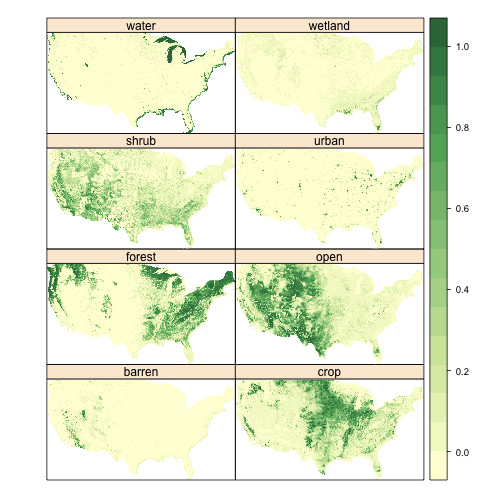
\includegraphics{fig_agc}
\end{center} 
\caption{Agland Complete cover maps} 
\label{fig:agc} 
\end{figure} 



blah blah blah

\begin{Schunk}
\begin{Sinput}
 setwd( rasterWd)  
 rmseDf <- 
   cbind( agland=c( TRUE, rep(FALSE, times=3)),
         rbind( c( TRUE, 0.5,
                  rmseRast( getPeelBand( aglandComplete, "crop"),
                           unstack( agland)[[ 1]]),
                  rmseRast( getPeelBand( aglandComplete, "open"),
                           unstack( agland)[[ 2]])),
               rmseDf))
 rmseDf <- within(rmseDf, offset <- as.logical( offset))
                                         # had to change offset column back
                                         # to true/false;  maybe this can be
                                         # avoided with list() instead of c()
 
 rmseXt <- xtable( rmseDf,
                  caption= "RMSE of Agland Complete vs. Agland2000",
                  label= "tab:rmse3",
                  digits= c( 0, 0, 0, 1, 3, 3))
                                         # looks like some kind of bug in xtable()
                                         # manual correction:
 rmseXt$agland <- rmseDf$agland
 rmseXt$offset <- rmseDf$offset
 print( rmseXt,
       include.rownames= FALSE,
       sanitize.colnames.function= function(x) x)
\end{Sinput}
% latex table generated in R 2.12.2 by xtable 1.5-6 package
% Wed Mar 16 16:57:49 2011
\begin{table}[ht]
\begin{center}
\begin{tabular}{llrrr}
  \hline
agland & offset & $A_{min}$ & $RMSE_{crop}$ & $RMSE_{open}$ \\ 
  \hline
TRUE & TRUE & 0.5 & 0.000 & 0.207 \\ 
  FALSE & TRUE & 0.5 & 0.150 & 0.235 \\ 
  FALSE & FALSE & 0.5 & 0.165 & 0.242 \\ 
  FALSE & FALSE & 1.0 & 0.180 & 0.267 \\ 
   \hline
\end{tabular}
\caption{RMSE of Agland Complete vs. Agland2000}
\label{tab:rmse3}
\end{center}
\end{table}\begin{Sinput}
 
\end{Sinput}
\end{Schunk}


\begin{Schunk}
\begin{Sinput}
 areasCt3 <- acreageTable( c( rasterNames2[ c( 1, 2, 4, 7)], "aglandComplete"))
 local({
   colnames( areasCt3) <- c( "Agland2000", "NLCD",
                            "\\pbox[c][][c]{3in}{MLCT\\\\No Mosaic}",
                            "\\pbox[c][][c]{3in}{\\smallskip{}MLCT\\\\Adjusted\\\\No Mosaic}",
                            "AgC")
   print( xtable( areasCt3 / 10^6, 
                 caption= "Agland Complete (AgC) acreages, $A_{min}=0.5$",
                 label= "tab:areas3",
                 digits= 1),
         size= "small",
         add.to.row= list( 
           pos= list( 0, nrow( areasCt)),
           command= rep("\\noalign{\\smallskip}", times= 2)),        
         sanitize.colnames.function= function(x) x)
   ##,
   ##      floating= FALSE)
 })
\end{Sinput}
% latex table generated in R 2.12.2 by xtable 1.5-6 package
% Wed Mar 16 16:57:55 2011
\begin{table}[ht]
\begin{center}
{\small
\begin{tabular}{rrrrrr}
  \hline
 & Agland2000 & NLCD & \pbox[c][][c]{3in}{MLCT\\No Mosaic} & \pbox[c][][c]{3in}{\smallskip{}MLCT\\Adjusted\\No Mosaic} & AgC \\ 
  \noalign{\smallskip} \hline
water & 0.0 & 96.5 & 74.3 & 98.0 & 98.7 \\ 
  forest & 0.0 & 513.2 & 410.8 & 346.4 & 365.6 \\ 
  shrub & 0.0 & 420.1 & 387.2 & 349.8 & 352.7 \\ 
  open & 557.1 & 429.6 & 538.7 & 515.9 & 472.9 \\ 
  wetland & 0.0 & 95.0 & 26.0 & 106.5 & 109.1 \\ 
  crop & 446.5 & 310.8 & 495.4 & 437.5 & 447.9 \\ 
  urban & 0.0 & 102.8 & 27.3 & 107.1 & 114.7 \\ 
  NA &  &  &  &  &  \\ 
  barren & 0.0 & 24.5 & 32.8 & 31.4 & 31.1 \\ 
  (all) & 1003.7 & 1992.5 & 1992.5 & 1992.5 & 1992.5 \\ 
   \noalign{\smallskip} \hline
\end{tabular}
}
\caption{Agland Complete (AgC) acreages, $A_{min}=0.5$}
\label{tab:areas3}
\end{center}
\end{table}\begin{Sinput}
 
 
\end{Sinput}
\end{Schunk}


\todo[inline,caption={Decide what to do with old code in Analysis
  chapter}]{The remaining code in this draft of the Analysis chapter
  has fallen out of date.  The maps are based on old data that has
  been replaced and the tables are probably not going to appear given
  that the code sections will not be evaluated.  The idea of finding
  correlations across a set of difference map still seems promising,
  so I am leaving it in the source code for now.}


To assess the impact of this step on the overall accuracy it is useful
compare the errors and biases of our newly derived ``Agland
Complete''(AgC) data set for all cover classes before and after the
adjustment of the cell-by-cell cropland areas to match Agland2000.





 

\begin{Schunk}
\begin{Sinput}
 ## calculate RMSE/bias summaries
 ## comparing everything to NLCD
 
 
 rmseAgc <- rmseSummary( function(c) paste(  "agc", c, sep="_"),
                        function(c) paste( "nlcd", c, sep="_"))
 rmseAs00 <- rmseSummary( function(c) paste( "mlct_2001", c, "As00", sep="_"),
                         function(c) paste( "nlcd", c, sep="_"))
 rmseAs05 <- rmseSummary( function(c) paste( "mlct_2001", c, "As05", sep="_"),
                         function(c) paste( "nlcd", c, sep="_"))
\end{Sinput}
\end{Schunk}

\begin{Schunk}
\begin{Sinput}
 ## t( rmseAgc)
 ## t( rmseAs00)
 ## t( rmseAs05)
 
 print( xtable( t( rmseAgc), 
               caption= "Errors and Biases of Aglands Complete relative to NLCD",
               label= "tab:ebagc",
               digits= c( 0, 2, -2, 0, 0)))
 print( xtable( t( rmseAs00), 
               caption= "Errors and Biases of MLCT, $A_s = 0.0$ relative to NLCD",
               label= "tab:ebmlct00",
               digits= c( 0, 2, -2, 0, 0)))
 print( xtable( t( rmseAs05), 
               caption= "Errors and Biases of MLCT, $A_s = 0.5$ relative to NLCD",
               label= "tab:ebmlct05",
               digits= c( 0, 2, -2, 0, 0)))
\end{Sinput}
\end{Schunk}

\begin{Schunk}
\begin{Sinput}
 ## agcAvgAcres <-
 ##   sapply( paste( "agc_", covers, sep=""),
 ##          function( map) {
 ##            mapRast <- raster( as.spgdf( handle( map)))
 ##            return( cellStats( areaAcres( mapRast), sum)
 ##                   /( ncell( mapRast) - cellStats( mapRast, 'countNA')))
 ##          })
 
 
 ## getting ready to plot
 
 stackAgc <- stackHandles( grepHandles(  "^agc"))
 attr( stackAgc, "layernames") <-  covers
 stackNlcd <- stackHandles( grepHandles( "^nlcd"))
 attr( stackNlcd, "layernames") <-  covers
 stackDiff <- stackAgc -stackNlcd
 attr( stackDiff, "layernames") <-  covers
 
\end{Sinput}
\end{Schunk}

\begin{figure} 
\begin{center} 

\begin{Schunk}
\begin{Sinput}
 ##spgdfNlcd <- as.spgdf( stackNlcd)
 ##names( spgdfNlcd) <- layerNames( stackNlcd)
 setwd( texWd)
 png( file="fig_nlcd.png")
 print( coverMaps( stackNlcd, 0.4))
 dev.off()
\end{Sinput}
\end{Schunk}

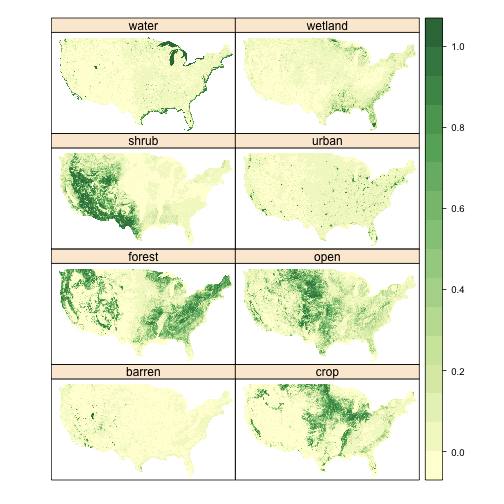
\includegraphics{fig_nlcd}
\end{center} 
\caption{NLCD cover maps} 
\label{fig:nlcd} 
\end{figure} 

\begin{figure} 
\begin{center} 

\begin{Schunk}
\begin{Sinput}
 ##spgdfDiff <- as.spgdf( stackDiff)
 ##names( spgdfDiff) <- layerNames( stackDiff)
 setwd( texWd)
 png( file="fig_diff.png")
 print( coverMaps( stackDiff, 0.4) + 
       scale_fill_gradientn( "diff", colours= rev( brewer.pal( 11, "BrBG")), 
                            limits= c( 0.1, -0.1),
                            breaks= seq( 0.1, -0.1, by= -0.02)))
 dev.off()
\end{Sinput}
\end{Schunk}

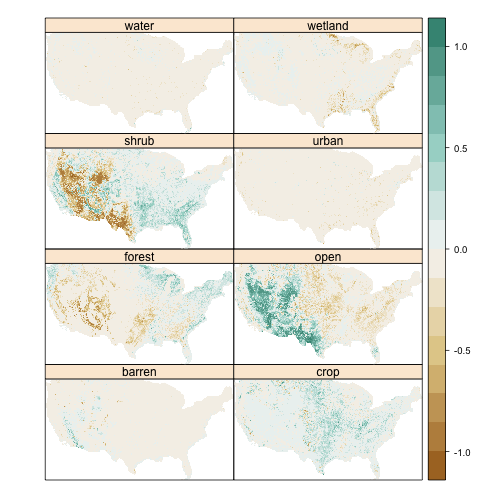
\includegraphics{fig_diff}
\end{center} 
\caption{Difference maps, Aglands Complete minus NLCD} 
\label{fig:diff} 
\end{figure} 

\begin{figure} 
\begin{center} 

\begin{Schunk}
\begin{Sinput}
 ## look for correlations across the difference maps
 
 corDiff <- cor( as.data.frame( as.spgdf( stackDiff))[,1:8])
 colnames( corDiff) <- unlist( lapply( 
                                      strsplit( colnames( corDiff), "\\."), 
                                      function( x) return( x[ 2])))
 rownames( corDiff) <- unlist( lapply( 
                                      strsplit( rownames( corDiff), "\\."), 
                                      function( x) return( x[ 2])))
 ord <- order.dendrogram( as.dendrogram( hclust( dist( corDiff))))
 corDiffPlot <- 
   ggplot( melt( corDiff),
          aes( x=X1, y=X2, fill= value)) +
   geom_tile() +
   theme_bw() +
   opts( panel.grid.minor= theme_blank(),
        panel.grid.major= theme_blank(),
        panel.background= theme_blank(),
        axis.title.x= theme_blank(),
        axis.text.x= theme_text( angle= 90, hjust=1),
        axis.title.y= theme_blank()) +
   scale_x_discrete( limits= colnames(corDiff)[ord]) +
   scale_y_discrete( limits= colnames(corDiff)[ord]) +
   scale_fill_gradientn( "cor", colours= rev( brewer.pal( 11, "BrBG")), 
                        limits= c( 1.0, -1.0),
                        breaks= seq( 1.0, -1.0, by= -0.2))
 setwd( texWd)
 png( file="fig_cordiff.png")
 print( corDiffPlot)
 dev.off()
\end{Sinput}
\end{Schunk}
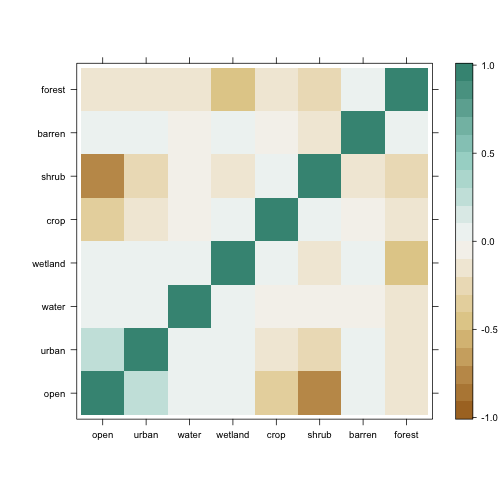
\includegraphics{fig_cordiff}
\end{center} 
\caption{Correlations across cover type in difference maps} 
\label{fig:cordiff} 
\end{figure} 

The elements of the matrix have been reordered according to the
clustering forumla given in \citet[sec. 6.2.3]{Sarkar2008} in order to
achieve a degree of visual clustering among the correlation vectors.

\begin{Schunk}
\begin{Sinput}
 options( prompt= "> ", continue= "+ ", width= 80)
\end{Sinput}
\end{Schunk}

%%% Local Variables: 
%%% mode: latex
%%% TeX-master: "thesis"
%%% End: 

